\documentclass[aspectratio=169,x11names]{beamer}
\usetheme{Pittsburgh}
\usepackage{xcolor}
\usepackage[utf8]{inputenc}
\usepackage{amsmath}
\usepackage{amsfonts}
\usepackage{amssymb}
\usepackage{graphicx}
\usepackage{multicol}
\usepackage{wrapfig}
\usepackage{hyperref}
\usepackage{tikz}
\usepackage{upgreek}
\usepackage[normalem]{ulem}
\usetikzlibrary{shapes,arrows,chains}

\author{Jonas Betzendahl}
\title{Metaverse - a telescope view into a different universe}

\beamertemplatenavigationsymbolsempty 

%src: https://tex.stackexchange.com/questions/34921/how-to-overlap-images-in-a-beamer-slide
\def\Put(#1,#2)#3{\leavevmode\makebox(0,0){\put(#1,#2){#3}}}

\definecolor{lightgray}{rgb}{0.75,0.75,0.75}
\definecolor{darkgray}{rgb}{0.2,0.2,0.2}
\definecolor{darkred}{rgb}{0.25,0,0}
\definecolor{darkgreen}{rgb}{0,0.25,0}
\definecolor{item}{rgb}{0.75,0.5,0.25}

\begin{document}

\setbeamercolor{background canvas}{bg=darkgray}
\setbeamercolor{itemize item}{fg=item}
\setbeamertemplate{itemize item}[square]

\setbeamercolor{normal text}{fg=lightgray}
\usebeamercolor[fg]{normal text}

\setbeamercolor{titlelike}{fg=lightgray}
\usebeamercolor[fg]{titlelike}

%------------------------------------------------------------------------------------
\section{Introduction}

\begin{frame}
\begin{center}
\vfill
\huge The Metaverse
\normalsize 
\smallskip
\smallskip

\dots a Telescope View into a Different Universe

\bigskip\bigskip\bigskip

\large Jonas Betzendahl\\
\texttt{@LambdaTotoro@chaos.social}\\
PwC Inspiration Hub\, 2023-09-14
\end{center}
\Put(330,0){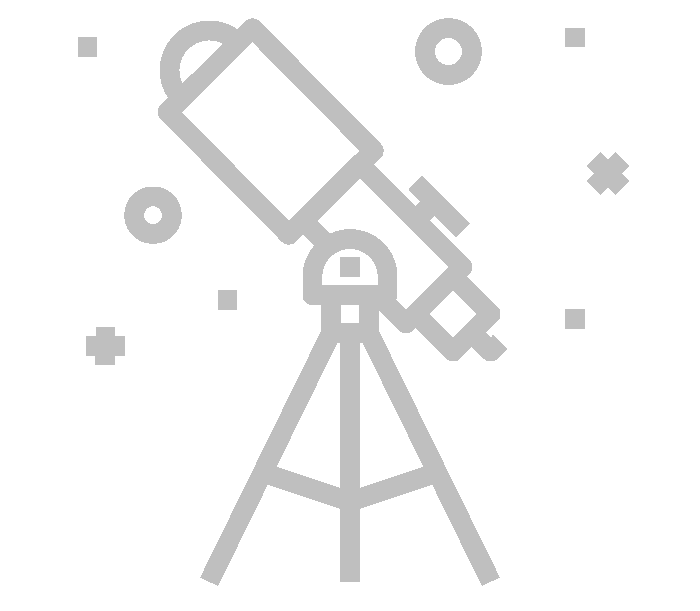
\includegraphics[width=0.2\textwidth,keepaspectratio]{images/noun-telescope.png} }
\end{frame}

\begin{frame}
\frametitle{Who am I?}
\begin{minipage}{0.45\textwidth}
\begin{center}

\includegraphics[height=0.8\textheight,keepaspectratio]{images/jonas} 
\end{center}
\end{minipage}%
\hfill
\begin{minipage}{0.55\textwidth}
\begin{itemize}
\item Jonas Betzendahl
\item \dots from Bielefeld
\item \dots Studies:
\begin{itemize}
\item Cognitive Informatics (B.Sc.)
\item Intelligent Systems (M.Sc.)
\end{itemize}
\item \dots Science Communication since 2016
\item \dots PhD Student in Informatics @ FAU Erlangen-Nürnberg (AI in Teaching)
\end{itemize}
\end{minipage}
\end{frame}

\begin{frame}
\frametitle{Who is this?}
\begin{minipage}{0.45\textwidth}
\begin{center}

\includegraphics[height=0.7\textheight,keepaspectratio]{images/cute_alien} 
\end{center}
\end{minipage}%
\hfill\pause
\begin{minipage}{0.55\textwidth}
\begin{itemize}
\item Q-t'$\forall$-l-ee-$\mathbb{N}$ (``cute alien'')
\item New to our sector of the milky way
\item Very curious, slightly naive
\item Wants to learn about the metaverse,\\ for some reason\dots
\end{itemize}
\end{minipage}
\end{frame}

%------------------------------------------------------------------------------------
\section{What IS the Metaverse?}

\begin{frame}
\begin{center}
\Large
Part I:\bigskip\\
\huge
What \emph{IS} the Metaverse?
\end{center}
\end{frame}

\subsection{Etymology}

\begin{frame}
\begin{center}

\includegraphics[height=0.825\textheight,keepaspectratio]{images/cute_alien_speech_meta.png} 
\end{center}
\end{frame}

\begin{frame}
\begin{center}

\includegraphics[height=0.825\textheight,keepaspectratio]{images/cute_alien_speech_not_meta.png} 
\end{center}
\end{frame}

\begin{frame}
\begin{minipage}{0.45\textwidth}
\begin{center}

\includegraphics[height=0.8\textheight,keepaspectratio]{images/snow-crash} 
\end{center}
\end{minipage}%
\begin{minipage}{0.55\textwidth}
\begin{center}
\end{center}
\end{minipage}
\end{frame}

\begin{frame}
\frametitle{Common Examples (1): VR Chat}
\begin{center}
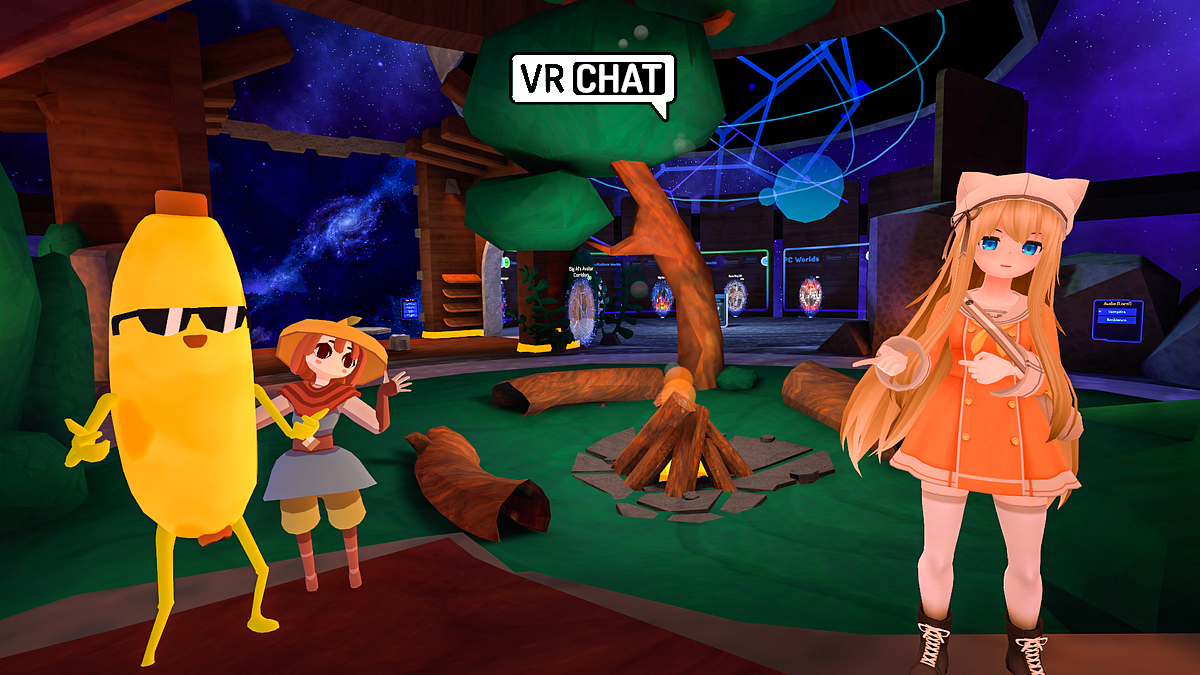
\includegraphics[height=0.8\textheight,keepaspectratio]{images/vr_chat} 
\end{center}
\end{frame}

\begin{frame}
\frametitle{Common Examples (2): Horizon Workrooms}
\begin{center}
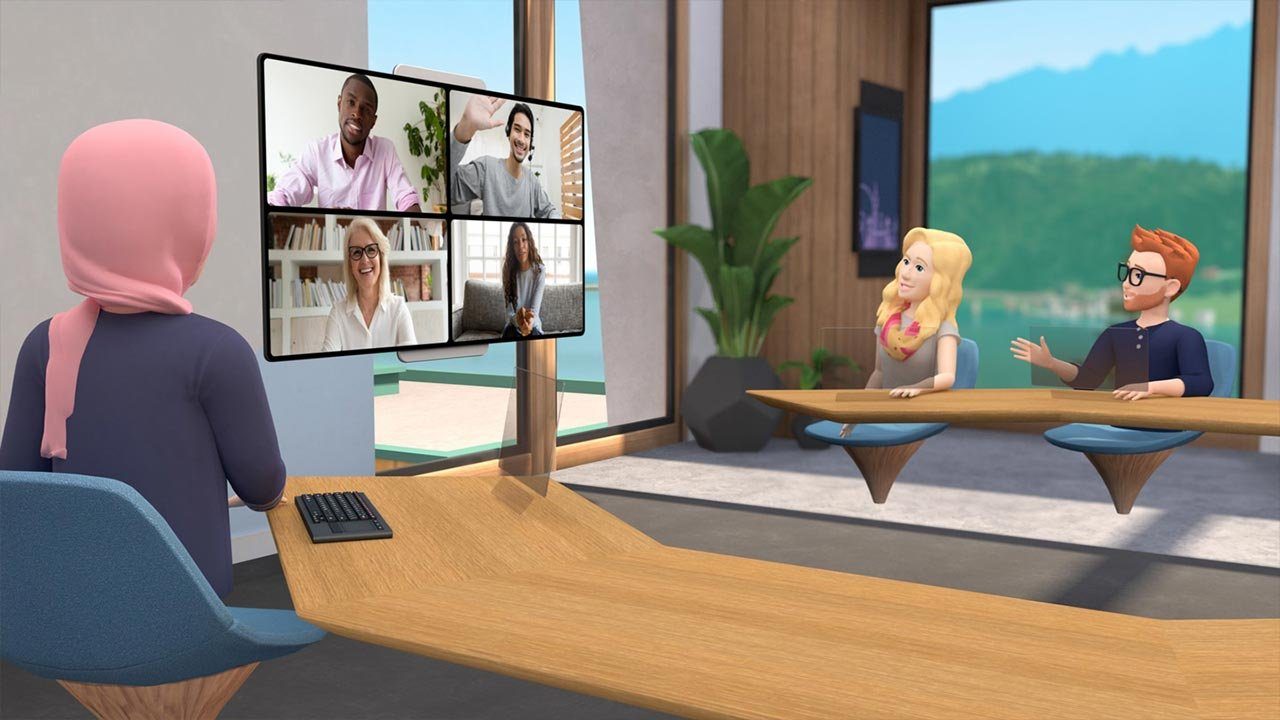
\includegraphics[height=0.8\textheight,keepaspectratio]{images/horizon_workrooms} 
\end{center}
\end{frame}

\begin{frame}
\frametitle{Definition Attempts}
There are \emph{many} different definitions of the Metaverse.\\
Here is one \emph{I} like:
\vfill

\begin{minipage}{0.65\textwidth}
``\emph{The} Metaverse \emph{is a collection of connected virtual spaces filled with digital object and agents (some controlled by users, some artificial) that allows for synchronous interactions.
\medskip

Often these spaces will be modelled after parts of the real world and incorporate avatars as representations of connected users.''}
\end{minipage}
\pause
\Put(0,0){
\includegraphics[width=0.4\textwidth,keepaspectratio]{images/cute_alien_speech_vague.png} }
\end{frame}

\begin{frame}
There are two broad perspectives on why any useful definition of the Metaverse tends
to be vague\dots\bigskip\bigskip\pause

\begin{minipage}{0.5\textwidth}
\begin{center}
\Large
\emph{cynical}
\normalsize\bigskip

The definition is vague because ``Metaverse'' is an industry buzzword without any
actual technical meaning.
\end{center}
\end{minipage}%
\begin{minipage}{0.5\textwidth}
\begin{center}
\Large
\emph{hopeful}
\normalsize\bigskip

The definition is vague because the idea is general and encompasses a large number of use cases, similar to the internet.
\end{center}
\end{minipage}

\Put(60,-220){
\includegraphics[width=0.2\textwidth,keepaspectratio]{images/cute_alien_cynical.png} }
\Put(260,-220){
\includegraphics[width=0.2\textwidth,keepaspectratio]{images/cute_alien_hopeful.png} }

\end{frame}

\begin{frame}
\frametitle{Timeline}
\begin{minipage}{0.33\textwidth}
\begin{center}
\begin{itemize}
\item 1972: Snow Crash coins the term
\end{itemize}
\end{center}
\end{minipage}%
\begin{minipage}{0.33\textwidth}
\begin{center}
\begin{itemize}
\item 1972: Snow Crash coins the term
\end{itemize}
\end{center}
\end{minipage}%
\begin{minipage}{0.33\textwidth}
\begin{center}
\begin{itemize}
\item 2021: Facebook rebrands as Meta
\end{itemize}
\end{center}
\end{minipage}%
\vfill
\begin{center}
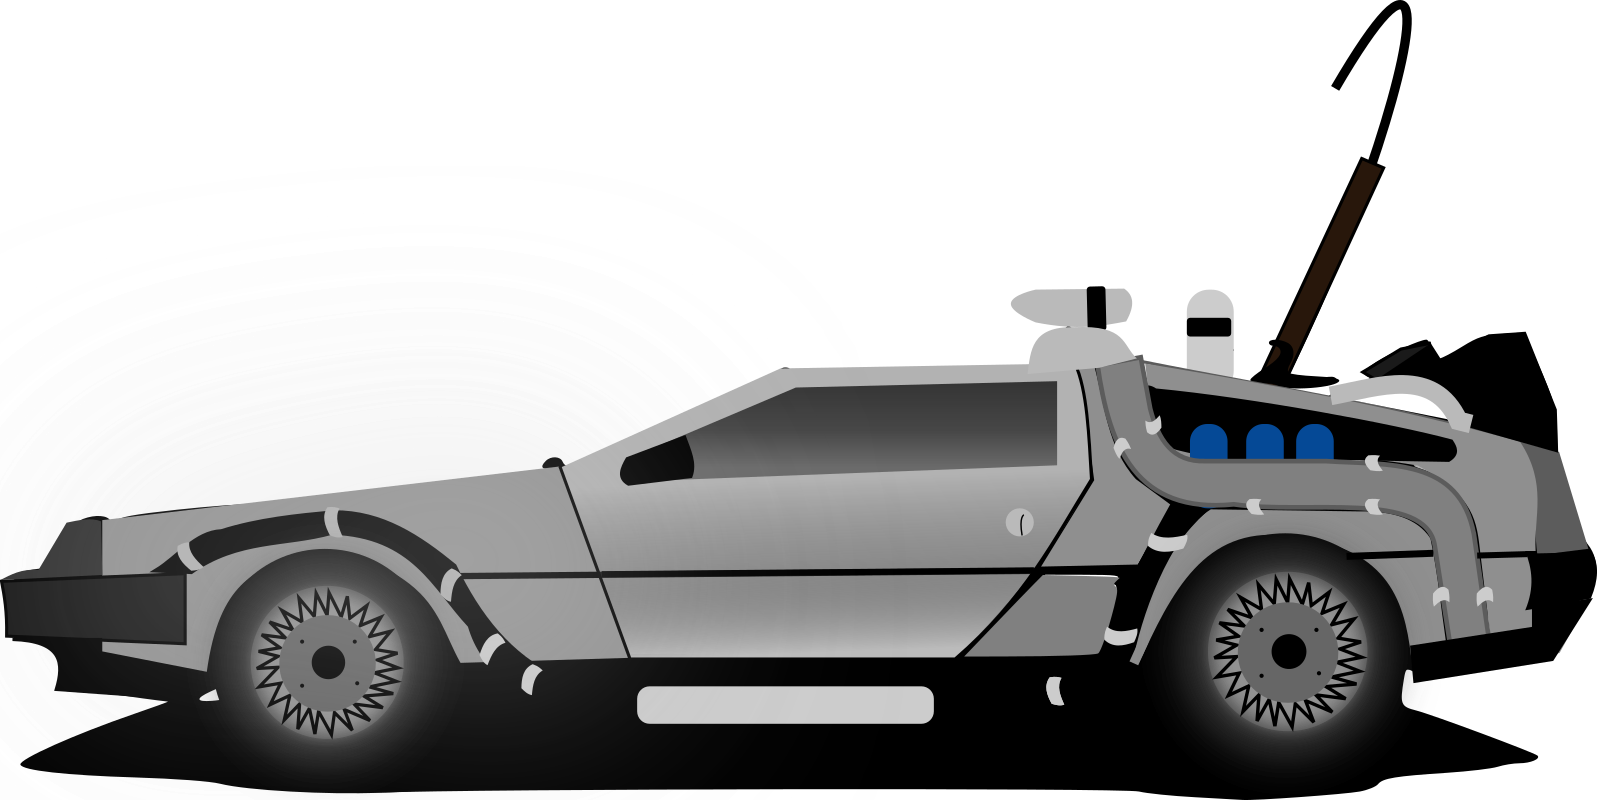
\includegraphics[height=0.3\textheight,keepaspectratio]{images/delorean.png} 
\end{center}
\end{frame}

%------------------------------------------------------------------------------------
\section{What ISN'T the Metaverse?}

\begin{frame}
\begin{center}
\Large
Part II:\bigskip\\
\huge
What \emph{ISN'T} the Metaverse?
\end{center}
\end{frame}

\subsection{Work only}

\begin{frame}
\begin{center}
\Large
Part II.1:\bigskip\\
\huge
The Metaverse is not\dots\\ only for work
\end{center}
\end{frame}


\begin{frame}
\begin{minipage}{0.45\textwidth}
\begin{center}

\includegraphics[width=\textwidth,keepaspectratio]{images/second_life_logo} 
\end{center}
\end{minipage}%
\begin{minipage}{0.55\textwidth}
\begin{center}
\end{center}
\end{minipage}
\end{frame}

\begin{frame}
\begin{minipage}{0.45\textwidth}
\begin{center}

\includegraphics[width=0.7\textwidth,keepaspectratio]{images/roblox_logo} 
\end{center}
\end{minipage}%
\begin{minipage}{0.55\textwidth}
\begin{center}
\end{center}
\end{minipage}
\end{frame}

\subsection{VR Headsets}

\begin{frame}
\begin{center}
\Large
Part II.2:\bigskip\\
\huge
The Metaverse is not\dots\\ only for VR headsets
\end{center}
\end{frame}

\begin{frame}
\begin{minipage}{0.55\textwidth}
\begin{center}
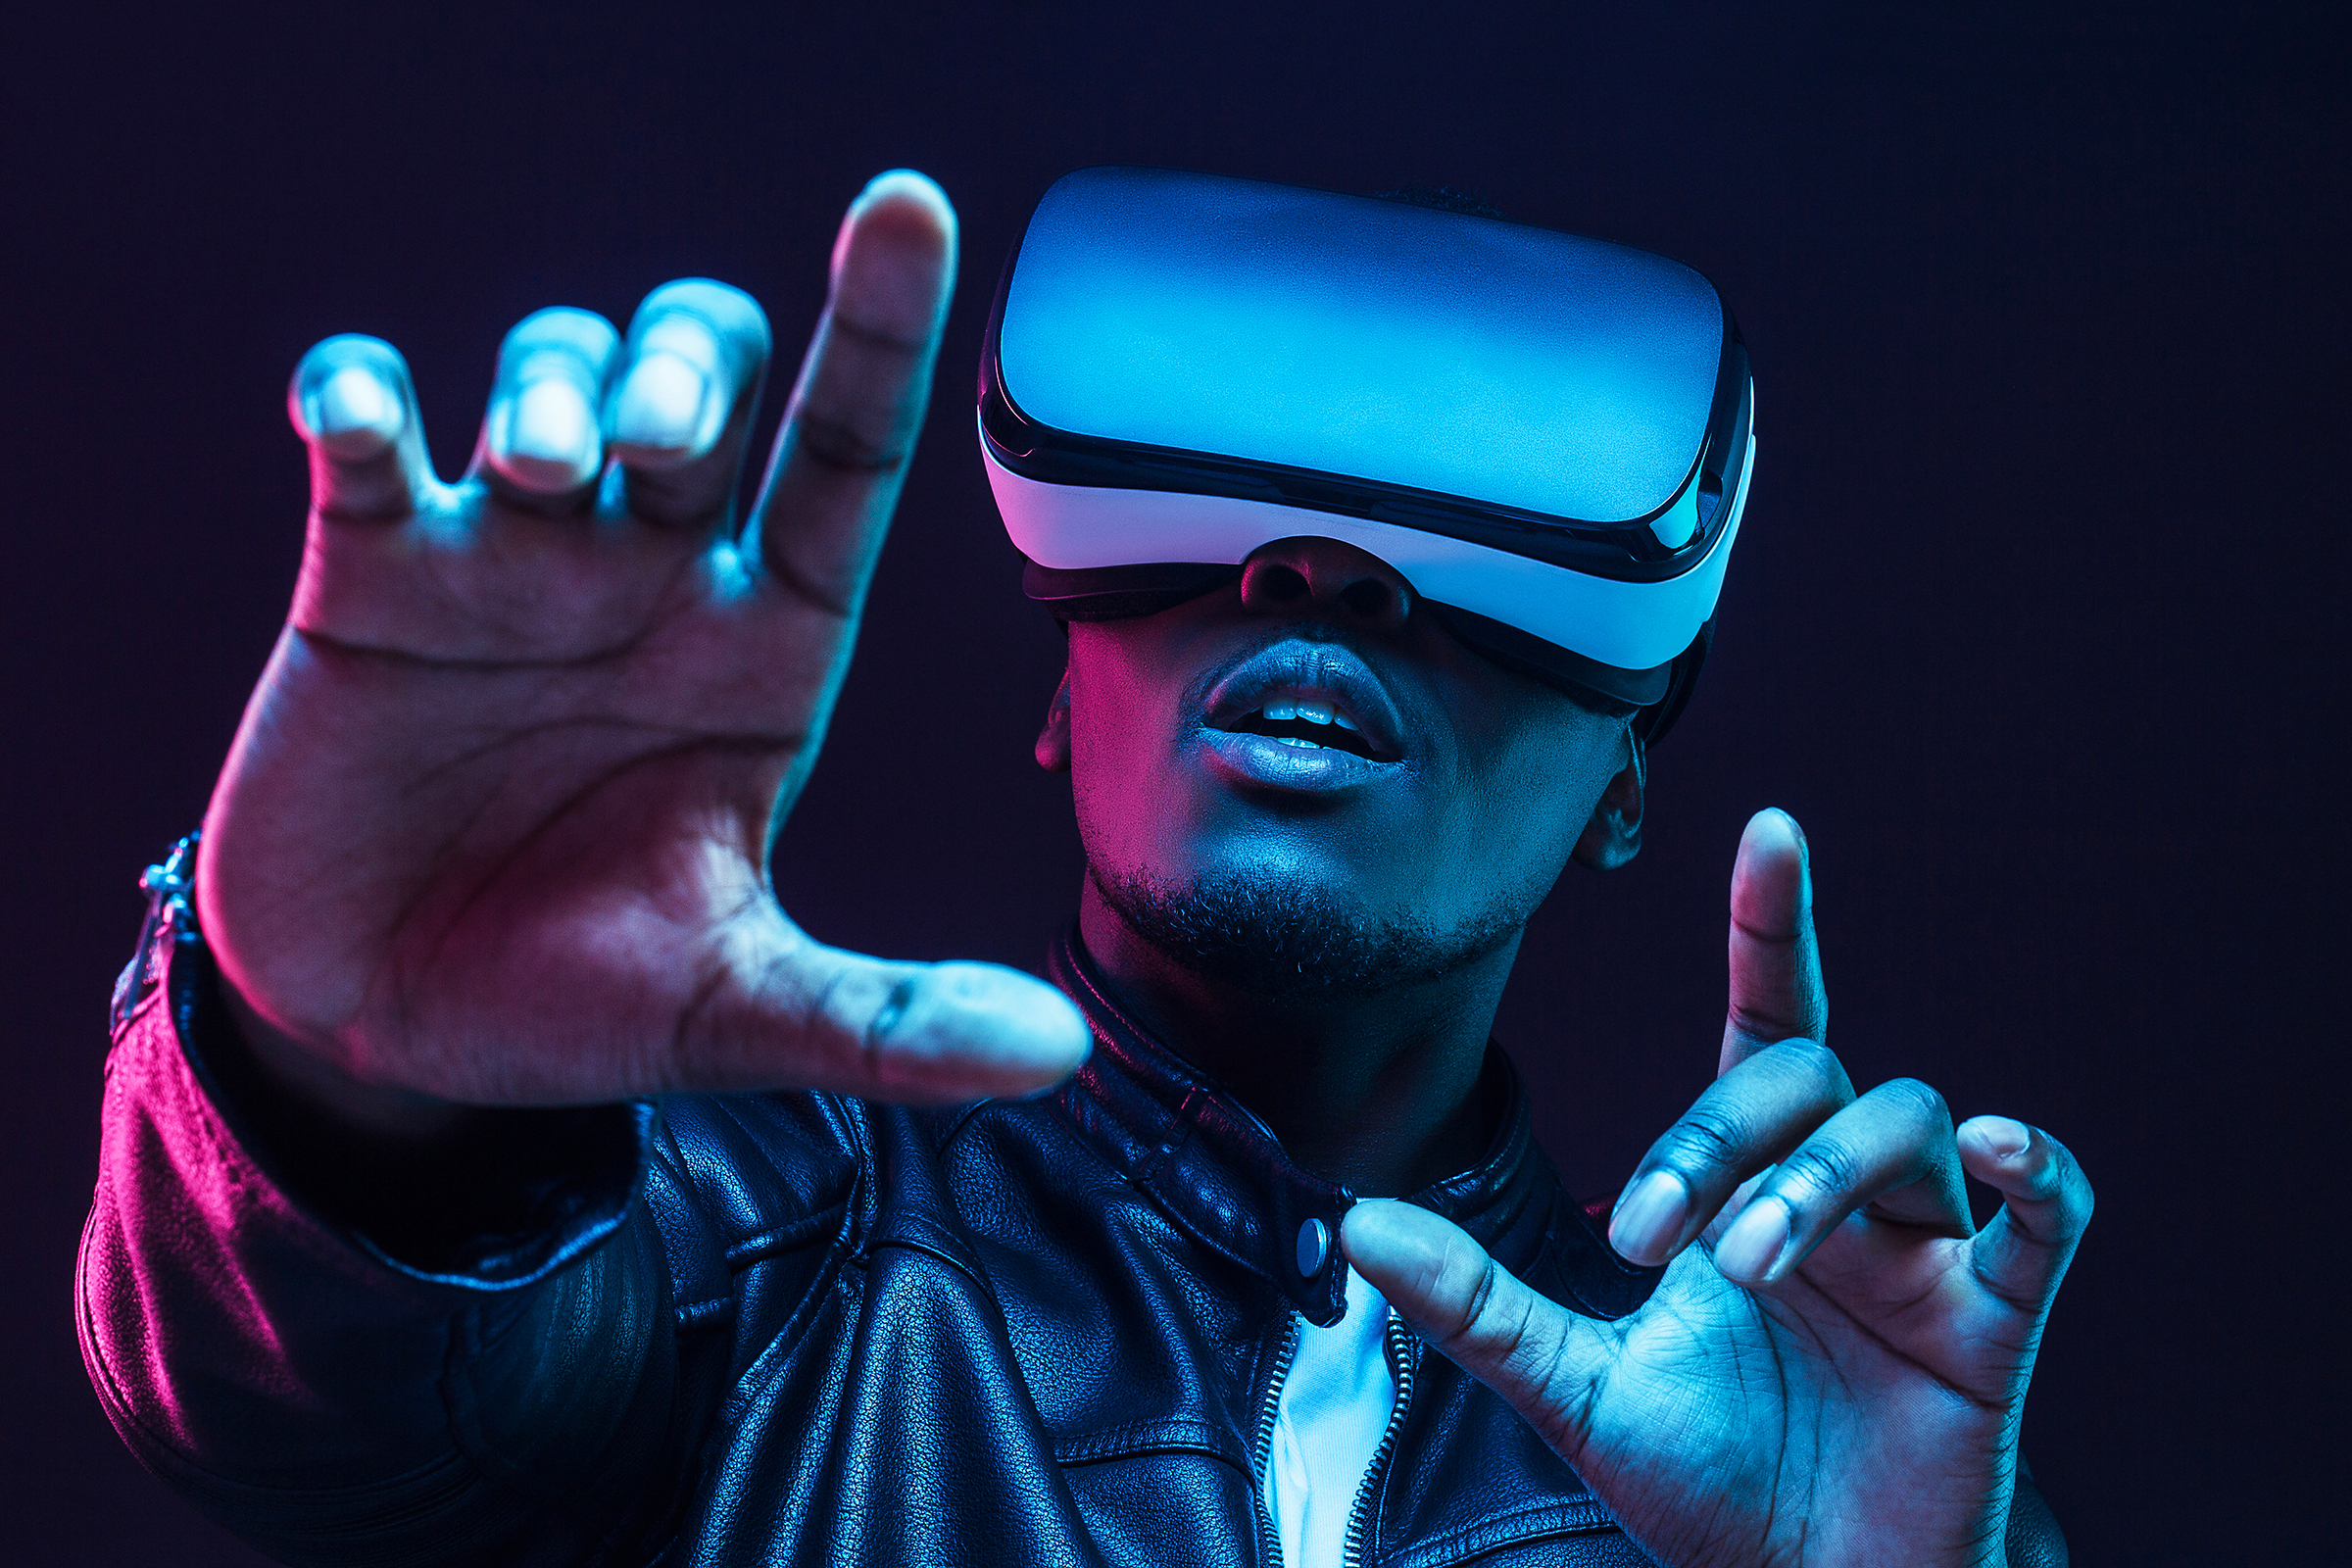
\includegraphics[width=0.8\textwidth,keepaspectratio]{images/stunning_vr_headset} 
\end{center}
\end{minipage}%
\begin{minipage}{0.45\textwidth}
We often think of \emph{this} when we think about the Metaverse. But in practice,
it can include a range of devices for both input and output and incorporate elements from:
\begin{itemize}
\item Augmented Reality
\item Mixed Reality
\item Virtual Reality
\end{itemize}
\end{minipage}
\end{frame}

\begin{frame}
\frametitle{Augmented Reality (1)}
\begin{center}
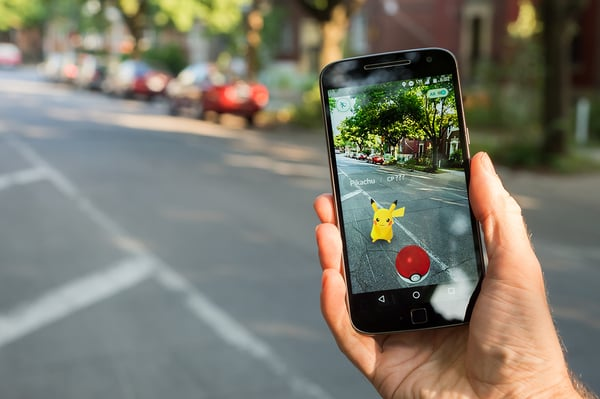
\includegraphics[width=0.7\textwidth,keepaspectratio]{images/pokemon-go-ar1} 
\end{center}
\pause
\Put(20,260){\rotatebox{-6}{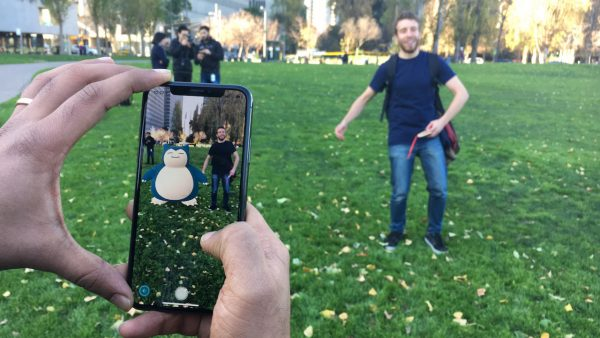
\includegraphics[width=0.85\textwidth,keepaspectratio]{images/pokemon-go-ar2}}}
\end{frame}

\begin{frame}
\frametitle{Augmented Reality (2)}
\begin{center}
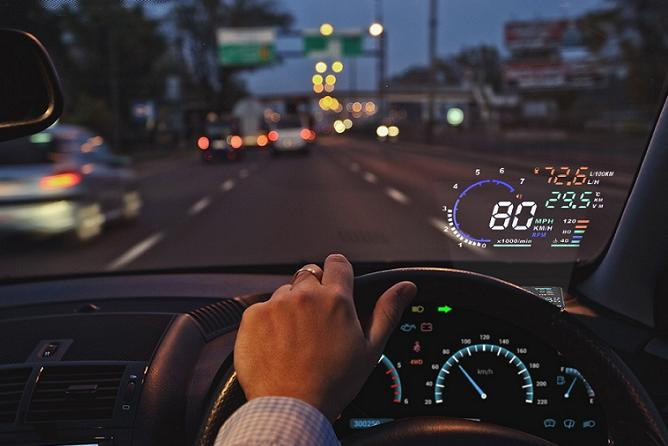
\includegraphics[height=0.8\textheight,keepaspectratio]{images/car_hud} 
\end{center}
\end{frame}

\begin{frame}
\frametitle{Mixed Reality (1)}
\begin{center}
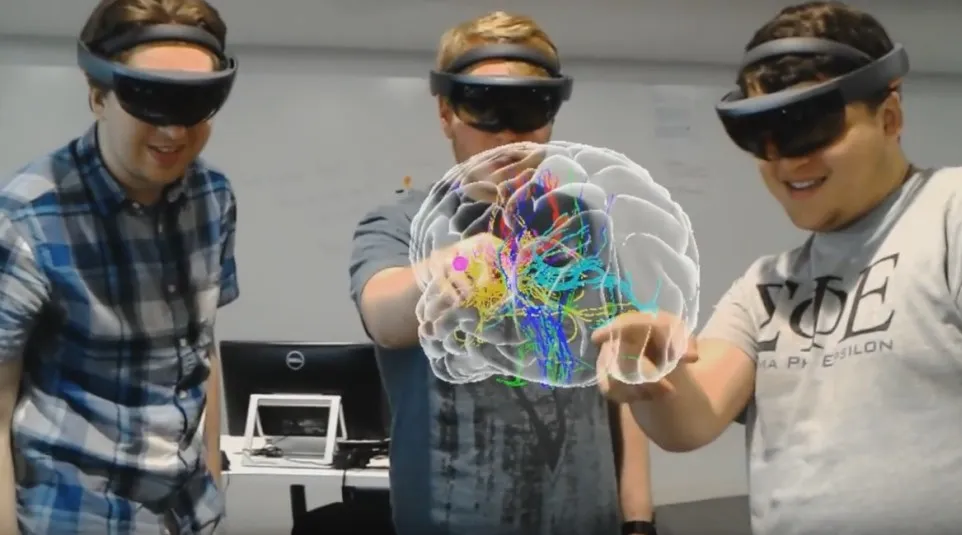
\includegraphics[height=0.8\textheight,keepaspectratio]{images/holo_anatomy} 
\end{center}
\end{frame}

\begin{frame}
\frametitle{Mixed Reality (2)}
\begin{center}
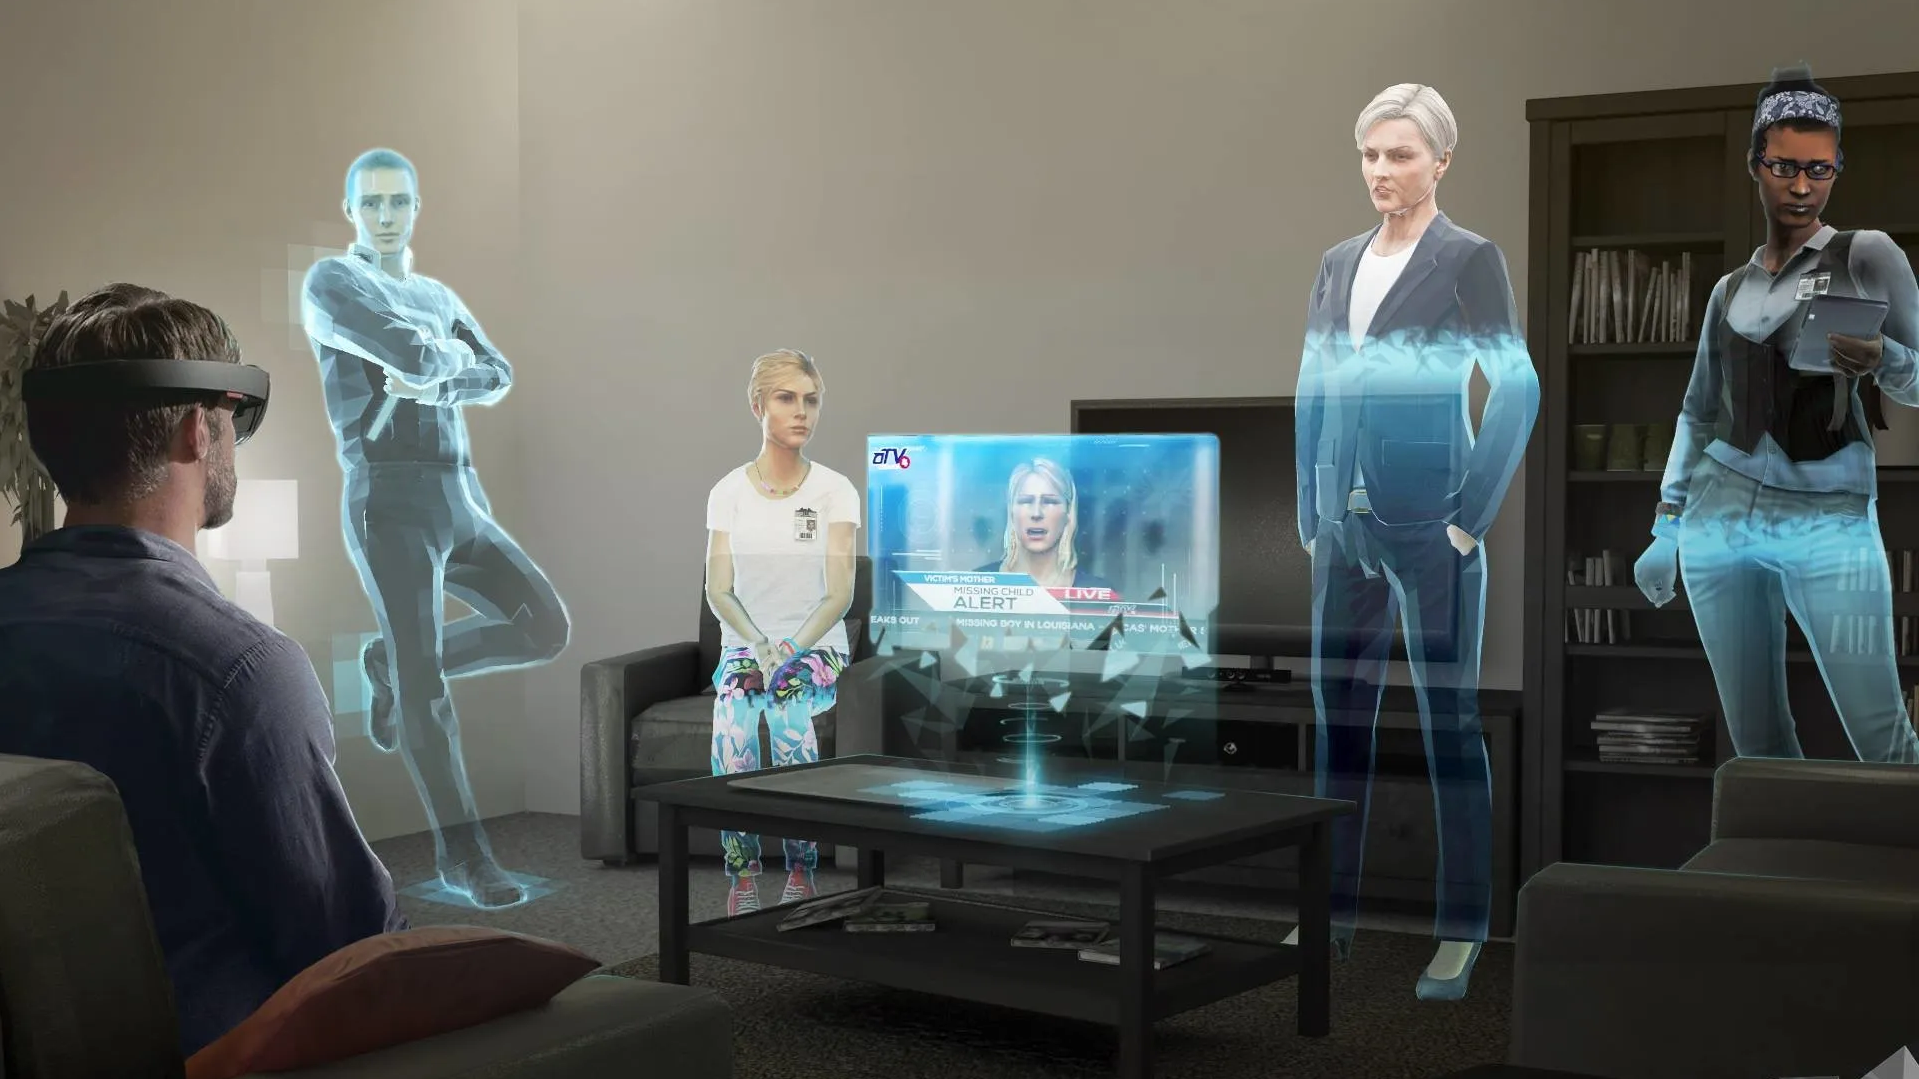
\includegraphics[height=0.8\textheight,keepaspectratio]{images/fragments} 
\end{center}
\end{frame}

\begin{frame}
\frametitle{Virtual Reality}
\end{frame}


\subsection{Built on the Blockchain}

\begin{frame}
\begin{center}
\Large
Part II.3:\bigskip\\
\huge
The Metaverse is not\dots\\ ``built on the blockchain''
\end{center}
\end{frame}

\begin{frame}
\frametitle{Tangent: What's a Blockchain, again?}
\end{frame}

\begin{frame}
\begin{center}
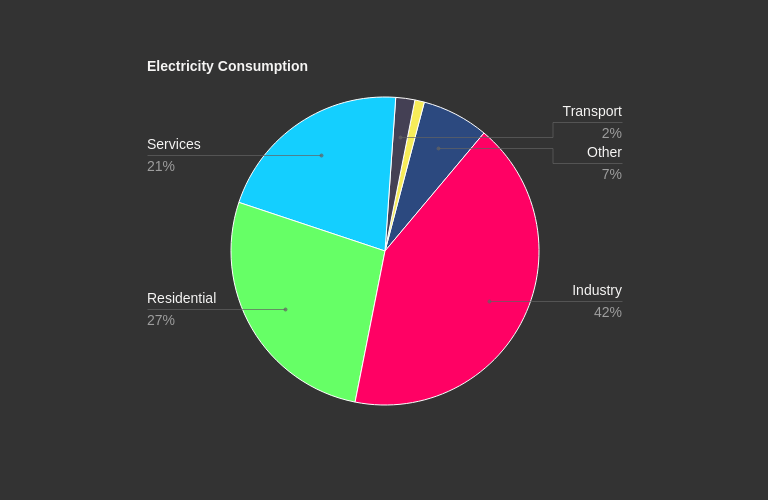
\includegraphics[height=0.95\textheight, keepaspectratio]{images/electricity_consumption} 
\end{center}
\end{frame}

%------------------------------------------------------------------------------------
\section{Science on the Metaverse}

\begin{frame}
\begin{center}
\Large
Part III:\bigskip\\
\huge
Science on the Metaverse
\end{center}
\end{frame}

\begin{frame}
\frametitle{Is there any science?}
It turns out to be difficult to find good scientific peer-reviewed research about the Metaverse, for a number of reasons:
\bigskip\bigskip

\begin{itemize}
\item very young field
\item wildly varying definitions
\item ``digital gold rush'' means lots of noise
\item good research usually in component-specific disciplines
\end{itemize}
\end{frame}

\begin{frame}
\frametitle{Scientists will \emph{never} shut up!}
However, there are some very helpful comment papers, like this one from the prestigious journal \textsc{Nature}\footnote{\url{https://doi.org/10.1038/s41562-023-01599-5}}:
\bigskip

\begin{center}
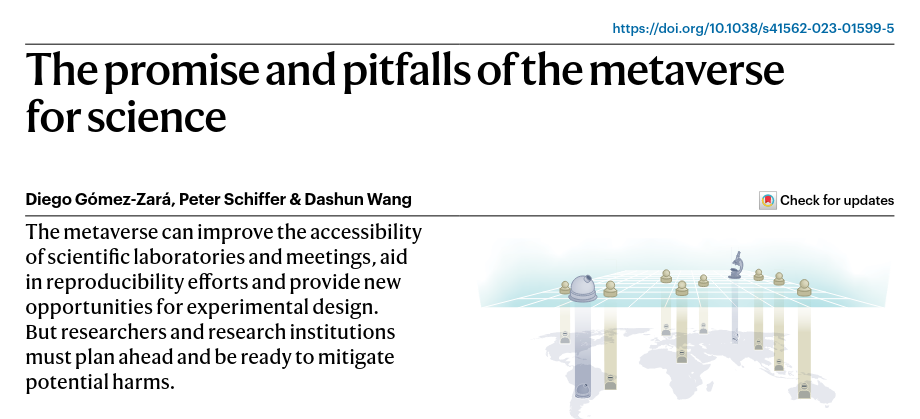
\includegraphics[width=0.8\textwidth,keepaspectratio]{images/nature_metaverse_paper.png} 
\end{center}
\end{frame}

\begin{frame}
\frametitle{Promises}
The paper lists promises of the Metaverse where it can shine:
\bigskip

\begin{itemize}
\item Accessibility
\item Reproducibility
\item Training \& Learning
\item New Environments
\end{itemize}
\end{frame}

\begin{frame}
\frametitle{Pitfalls}
The paper also lists challenges to look out for:
\bigskip

\begin{itemize}
\item Health Issues
\item Corporate Control
\item Code Fidelity
\item Resource Disparities
\item Privacy \& Surveillance
\item Biases \& Discrimination
\end{itemize}
\end{frame}

%------------------------------------------------------------------------------------
\section{The future of the Metaverse?}

\begin{frame}
\begin{center}
\Large
Part IV:\bigskip\\
\huge
The future of the Metaverse?
\end{center}
\end{frame}

\begin{frame}
\Large
\sout{Brutal} Radical Honesty Time:\bigskip\bigskip\pause

\begin{center}
\emph{It is my opinion that there is} \underline{no}\\
\emph{Metaverse Revolution just around the corner.}\bigskip\pause

\emph{The concept is ill-defined if it is supposed to go beyond\\
a) the hype of people selling the hopes of quick riches and\\
b) useful but already existing AR, MR \& VR technologies.}
\end{center}
\end{frame}

\begin{frame}
\frametitle{The Hype Cycle}
\begin{center}
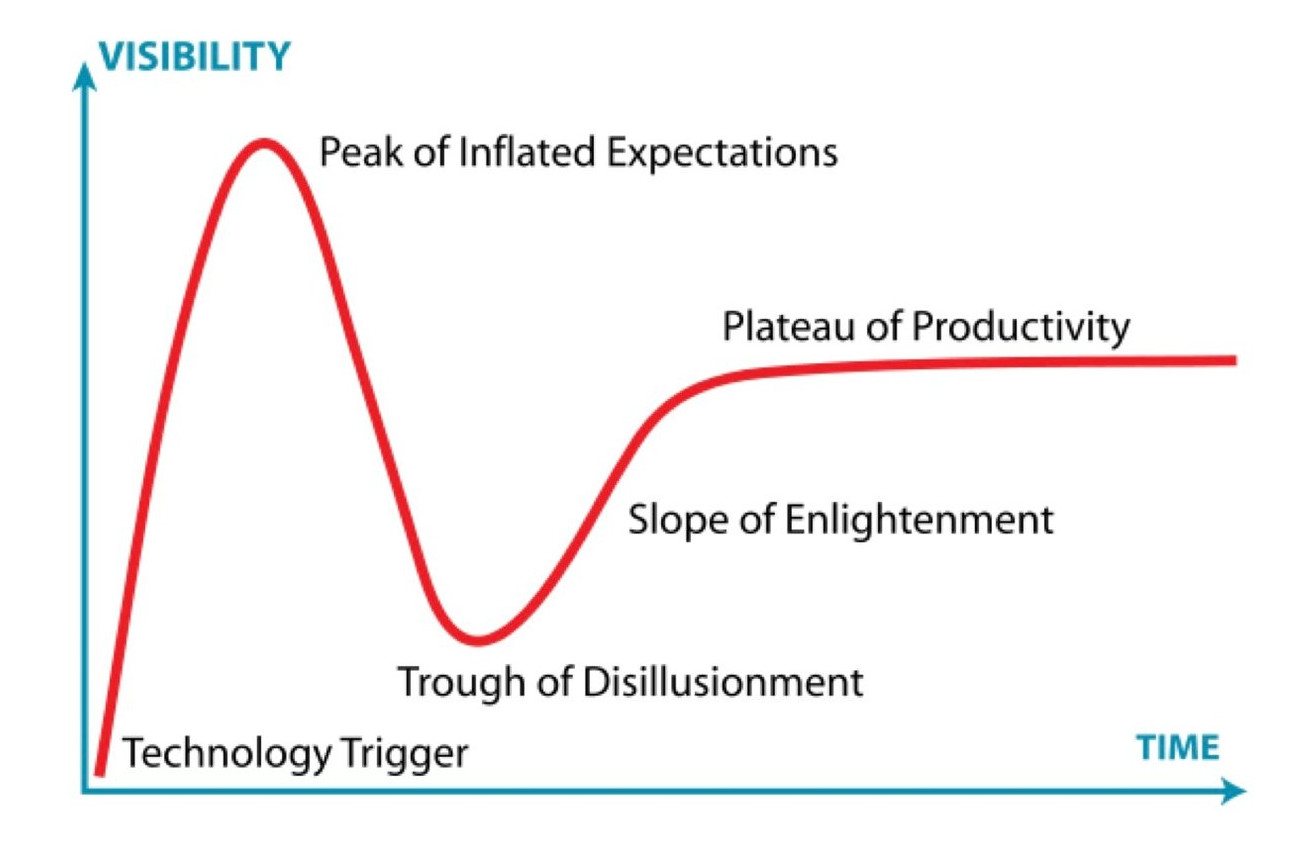
\includegraphics[height=0.7\textheight,keepaspectratio]{images/hype_cycle.jpg} 
\end{center}
\end{frame}

\begin{frame}
\begin{center}
\Huge
\emph{\dots BUT !}
\end{center}
\end{frame}

%------------------------------------------------------------------------------------
\section{End}
{
    \usebackgroundtemplate{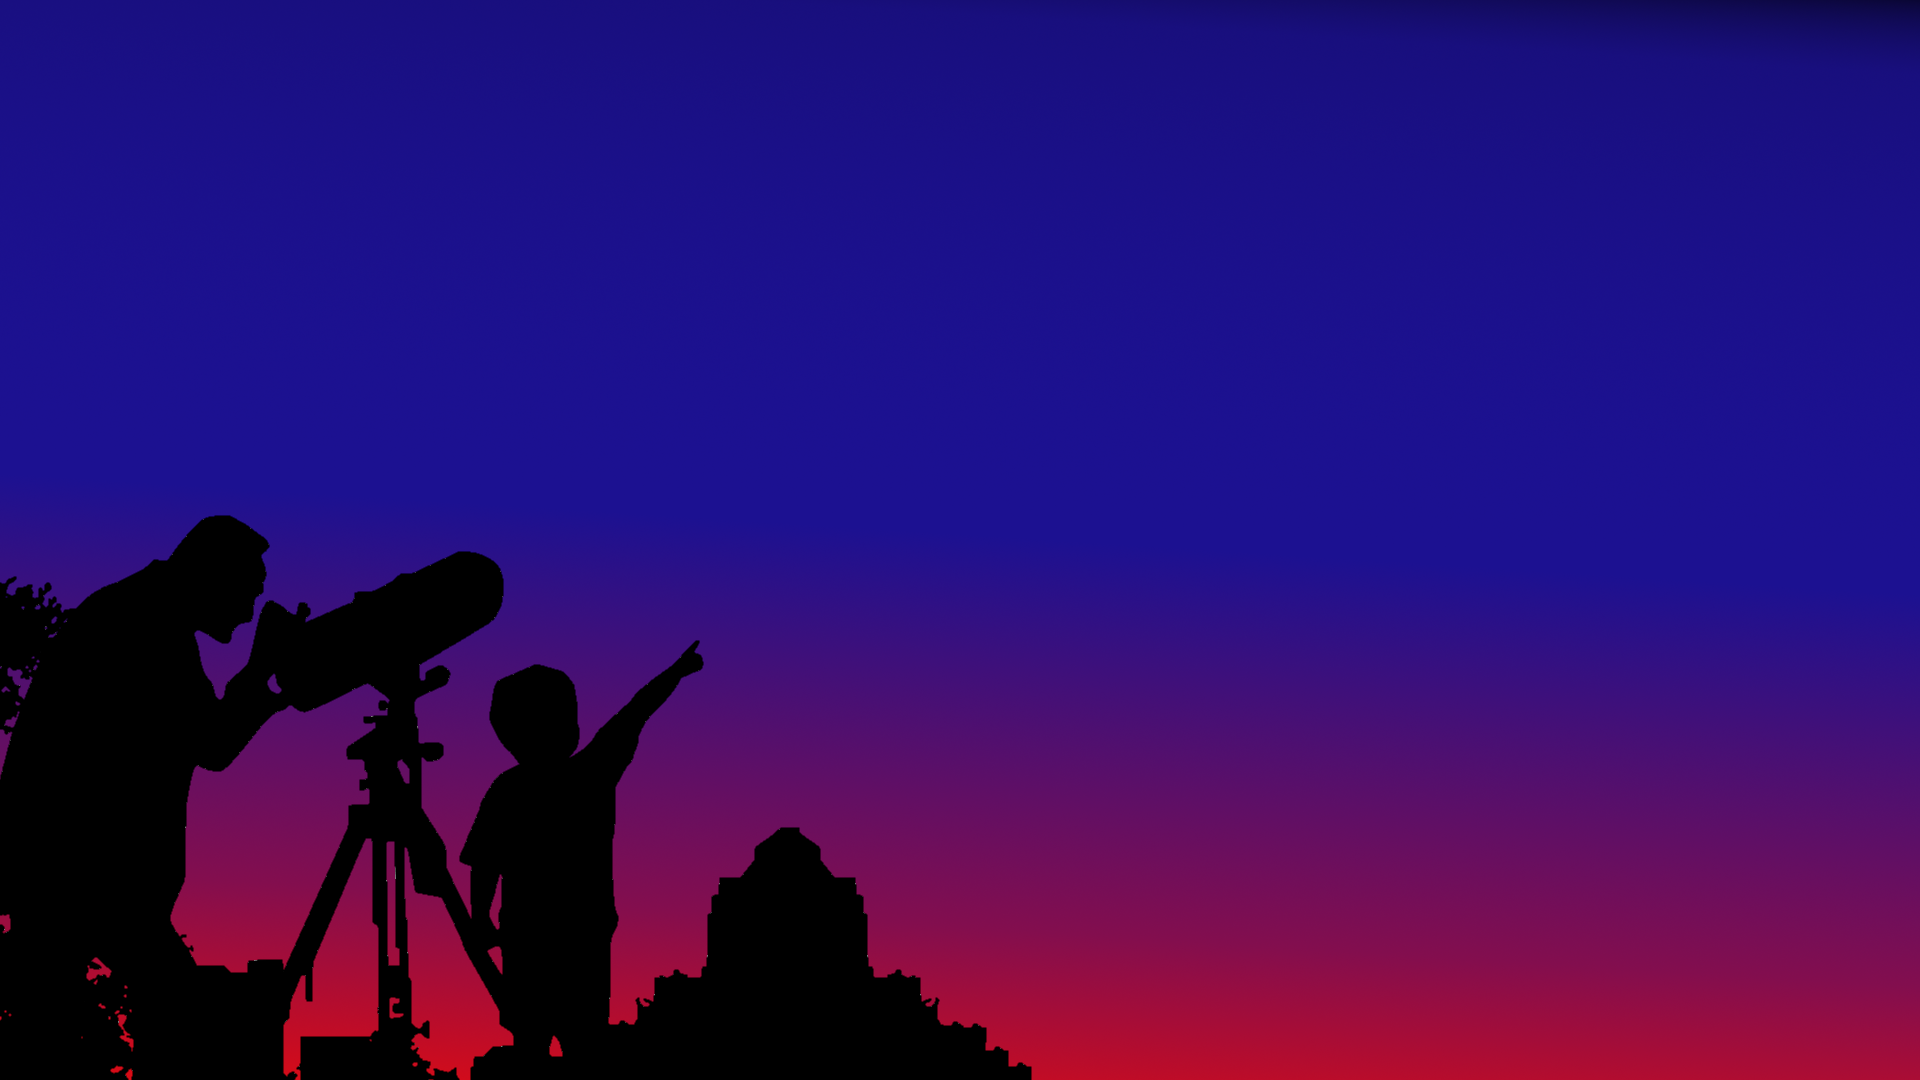
\includegraphics[height=\paperheight,width=\paperwidth]{images/sources}}
    \setbeamertemplate{navigation symbols}{}
    
    \begin{frame}
	\frametitle{Conclusions}
	\end{frame}
    
    \begin{frame}[fragile]
    \frametitle{Sources}
    ``The promise and pitfalls of the metaverse for science''
	\url{https://www.nature.com/articles/s41562-023-01599-5}
	\bigskip
    
    ``Metaverse beyond the hype: Multidisciplinary perspectives on emerging challenges, opportunities, and agenda for research, practice and policy''
    \url{https://doi.org/10.1016/j.ijinfomgt.2022.102542}
    \vfill
    \end{frame}
}

\end{document}

